\documentclass[11pt,a4paper]{article}

\usepackage{main}
\usepackage{cours}

\renewcommand{\typedocument}{Cours}
\renewcommand{\classe}{6e}
\renewcommand{\titre}{Méthode de calcul du triangle}

\begin{document}

\creertitre{Méthode de calcul du triangle}

\partie{Déterminer v à partir de d et t}

\begin{minipage}{12cm}
    On connait la formule \important{$v = d / t$}.
    \vspace{15pt}

    \exemple{Un athlète court $\SI{100}{\meter}$ en $\SI{10}{\second}$, quelle est sa vitesse ?\\[10pt]
        $d = \SI{100}{\meter}$ , $t = \SI{10}{\second}$ ,\\[10pt]
        $v = d / t = \frac{\SI{100}{\meter}}{\SI{10}{\second}} = \SI{10}{\meter/\second}$\\[10pt]
        La vitesse de l'athlète est de $\SI{10}{\meter/\second}$.
    }
\end{minipage}
\hfill
\begin{minipage}{8cm}
    
\includegraphics[width=5cm]{images/vitesse.png}
\end{minipage}

\partie{Déterminer d à partir de v et t}

\begin{minipage}{12cm}
    A l'aide du triangle, on trouve la formule \important{$d = v \times t$}.
    \vspace{15pt}

    \exemple{Un ballon roule à une vitesse de $\SI{5}{\meter/\second}$ pendant $\SI{3}{\second}$, quelle distance parcourt-il ?\\[10pt]
        $v = \SI{5}{\meter/\second}$ , $t = \SI{3}{\second}$ ,\\[10pt]
        $d = v \times t = \SI{5}{\meter/\second} \times \SI{3}{\second} = \SI{15}{\meter}$\\[10pt]
        La distance parcourue par le ballon est de $\SI{15}{\meter}$.
    }
\end{minipage}
\hfill
\begin{minipage}{8cm}
    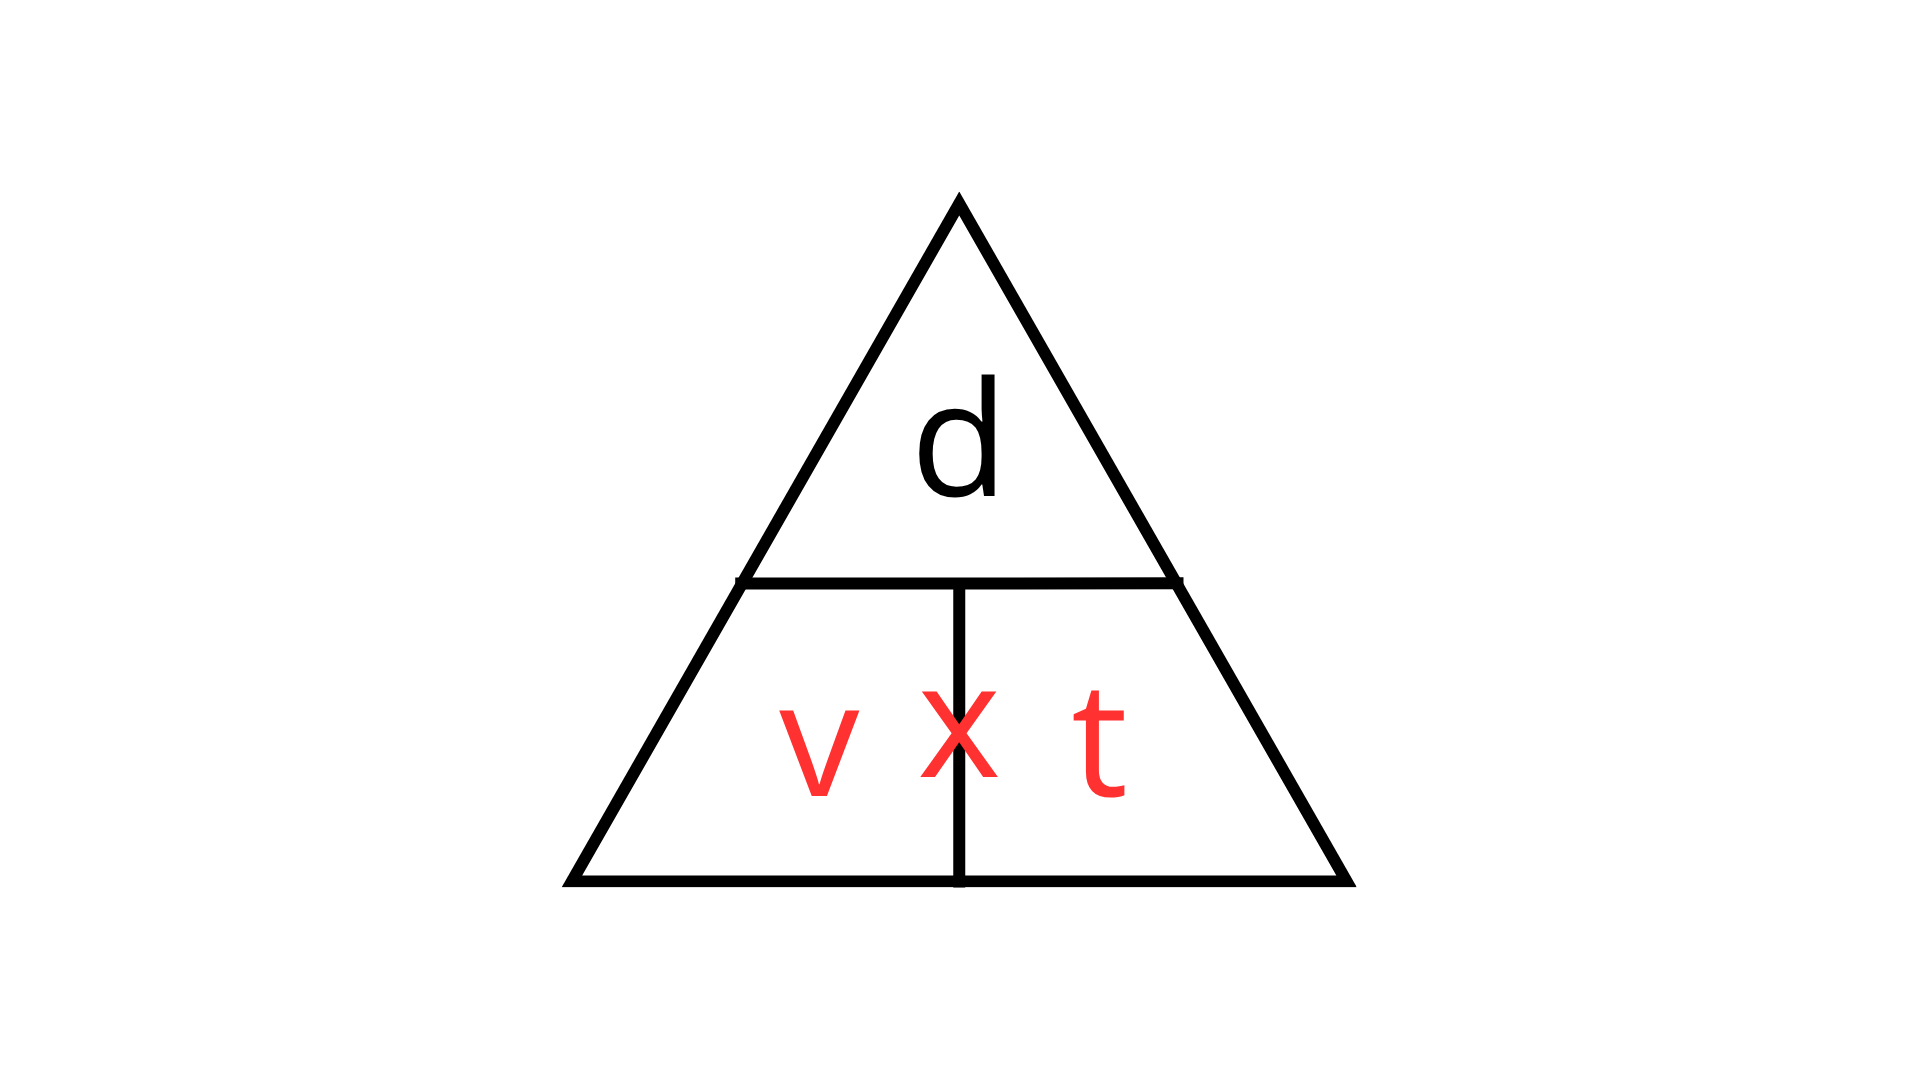
\includegraphics[width=5cm]{images/distance.png}
\end{minipage}

\partie{Déterminer t à partir de d et v}

\begin{minipage}{12cm}
    A l'aide du triangle, on trouve la formule \important{$t = d / v$}.
    \vspace{15pt}
    
    \exemple{Une voiture roule à $\SI{50}{\kilo\meter/\hour}$. Combien de temps met-elle pour parcourir $\SI{200}{\kilo\meter}$ ?\\[10pt]
        $d = \SI{200}{\kilo\meter}$ , $v = \SI{50}{\kilo\meter/\hour}$ ,\\[10pt]
        $t = d / v = \frac{\SI{200}{\kilo\meter}}{\SI{50}{\kilo\meter/\hour}} = \SI{4}{\hour}$\\[10pt]
        La voiture met 4 heures pour parcourir 200 km.
    }
\end{minipage}
\hfill
\begin{minipage}{8cm}
    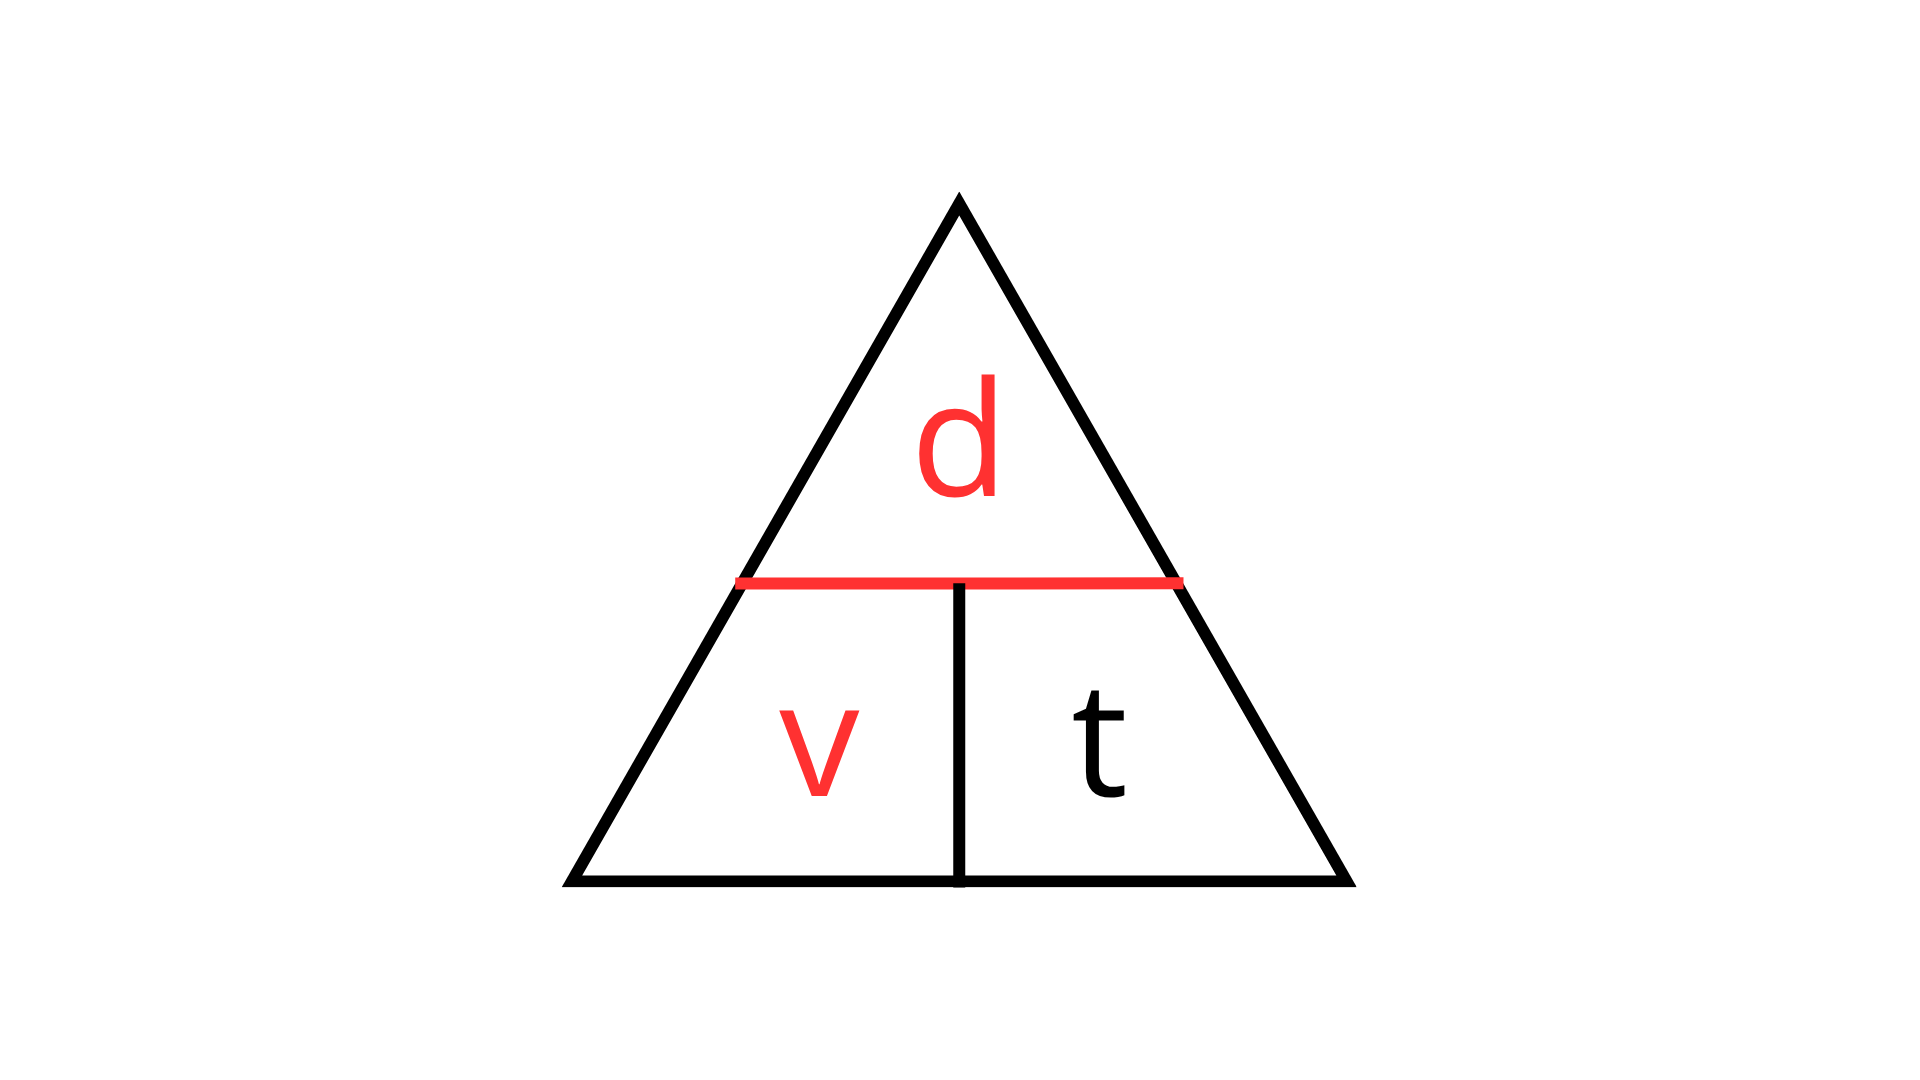
\includegraphics[width=5cm]{images/temps.png}
\end{minipage}

\partie{Autres utilisations du triangle}

La méthode du triangle peut aussi être utilisée avec d'autres formules de physique-chimie, comme la masse volumique ($\rho = m / V$).

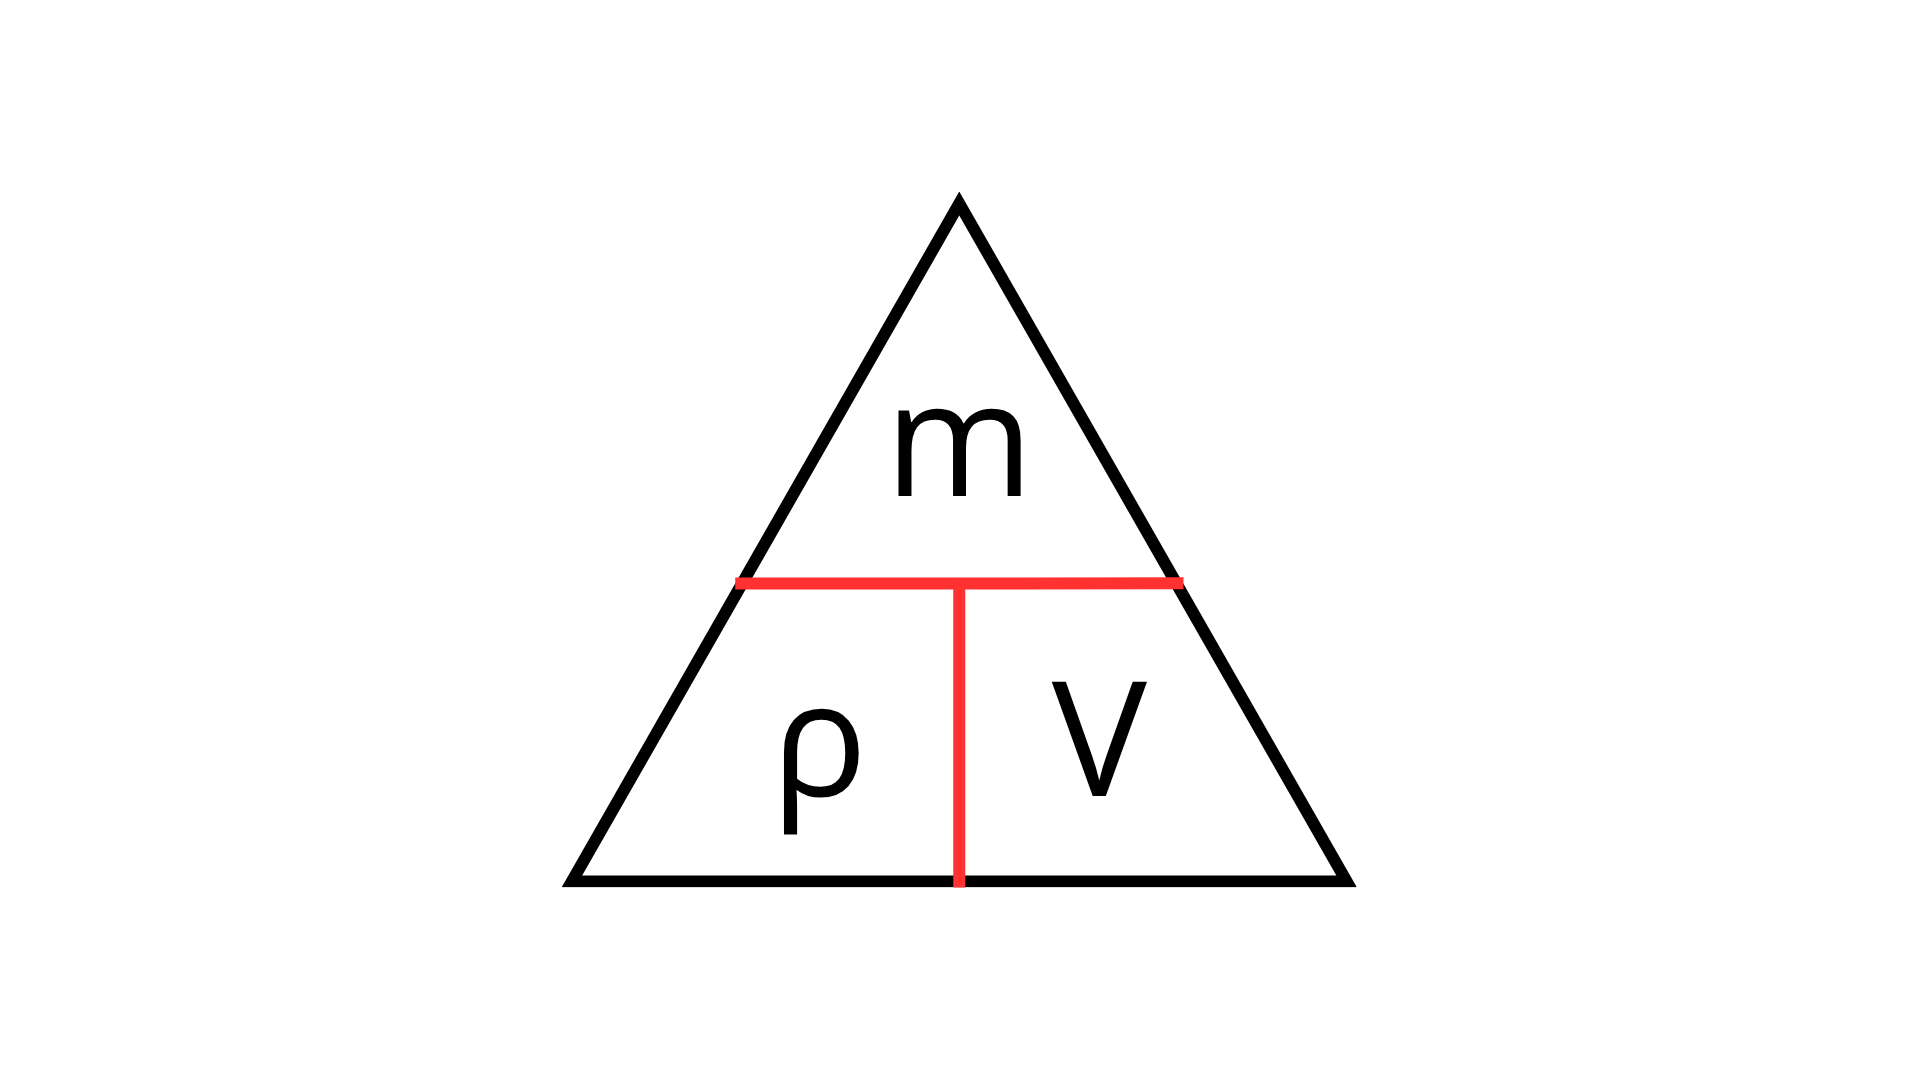
\includegraphics[width=5cm]{images/masse volumique.png}

\end{document}